%
% CSE Electronic Homework Template
% Last modified 8/23/2018 by Jeremy Buhler

\documentclass[11pt]{article}
\usepackage[left=0.7in,right=0.7in,top=1in,bottom=0.7in]{geometry}
\usepackage{fancyhdr} % for header
\usepackage{graphicx} % for figures
\usepackage{amsmath}  % for extended math markup
\usepackage{amssymb}
\usepackage[bookmarks=false]{hyperref} % for URL embedding
\usepackage[noend]{algpseudocode} % for pseudocode
\usepackage[plain]{algorithm} % float environment for algorithms

%%%%%%%%%%%%%%%%%%%%%%%%%%%%%%%%%%%%%%%%%%%%%%%%%%%%%%%%%%%%%%%%%%%%%%
% STUDENT: modify the following fields to reflect your
% name/ID, the current homework, and the current problem number

% Example: 
%\newcommand{\StudentName}{Jeremy Buhler}
%\newcommand{\StudentID{123456}

\newcommand{\StudentName}{Dingyu Wang (Howard)}
\newcommand{\StudentID}{COMP 642: Machine Learning}
\newcommand{\HomeworkNumber}{6}

%%%%%%%%%%%%%%%%%%%%%%%%%%%%%%%%%%%%%%%%%%%%%%%%%%%%%%%%%%%%%%%%%%%%%%%%
% You can pretty much leave the stuff up to the next line of %%'s alone.

% create header and footer for every page
\pagestyle{fancy}
\fancyhf{}
\lhead{\textbf{\StudentName}}
\chead{\textbf{\StudentID}}
\rhead{\textbf{HW \HomeworkNumber}}
\cfoot{\thepage}

% preferred pseudocode style
\algrenewcommand{\algorithmicprocedure}{}
\algrenewcommand{\algorithmicthen}{}

% ``do { ... } while (cond)''
\algdef{SE}[DOWHILE]{Do}{doWhile}{\algorithmicdo}[1]{\algorithmicwhile\ #1}%

% ``for (x in y ... z)''
\newcommand{\ForRange}[3]{\For{#1 \textbf{in} #2 \ \ldots \ #3}}

% these are common math formatting commands that aren't defined by default
\newcommand{\union}{\cup}
\newcommand{\isect}{\cap}
\newcommand{\ceil}[1]{\ensuremath \left\lceil #1 \right\rceil}
\newcommand{\floor}[1]{\ensuremath \left\lfloor #1 \right\rfloor}

%%%%%%%%%%%%%%%%%%%%%%%%%%%%%%%%%%%%%%%%%%%%%%%%%%%%%%%%%%%%%%%%%%%%%%
\usepackage[utf8]{inputenc}
\usepackage[english]{babel}
\setlength{\parindent}{0em}
\setlength{\parskip}{1em}
 \usepackage{pythonhighlight}
\usepackage{graphicx}
\graphicspath{ {./images/} }


\begin{document}
1) \\
a) \\
True positive rate = true positive / (true positive + false negative) \\
=  250/ (250 + 50) = 0.833 \\
False positive rate = false positive / (false positive + true negative) \\
= 50 / (50 + 250) = 0.166 \\
Positon Roc (FPR, TPR)=(0.166, 0.833) \\

b) \\
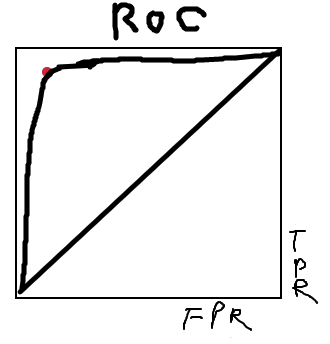
\includegraphics[scale=0.45]{roc}

c) \\
True positive rate = true positive / (true positive + false negative) \\
=  200/ (200 + 100) = 0.666 \\
False positive rate = false positive / (false positive + true negative) \\
= 100 / (100 + 200) = 0.333 \\
Positon Roc (FPR, TPR)=(0.333, 0.666) \\

d) \\
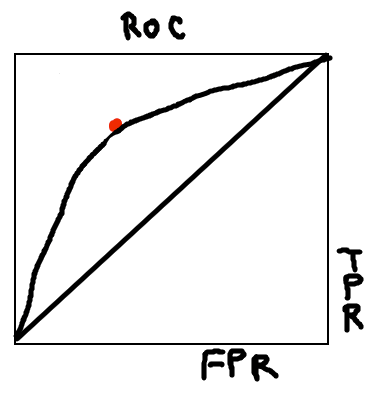
\includegraphics[scale=0.45]{roc2}

e) \\ 
The first model is clearly better. The model better separates the blue and red. The second model has a lot more false positive and false negatives. Also the ROC curve on the second model is a lot flatter, which means it's closer to just randomly guessing. 

f) \\
I think making the decision boundary 0.5 is a good choice. The 2 distributions are symmetric and 0.5 is right in the middle of the overlap. There is an equal number of false positives and false negatives.

2) \\
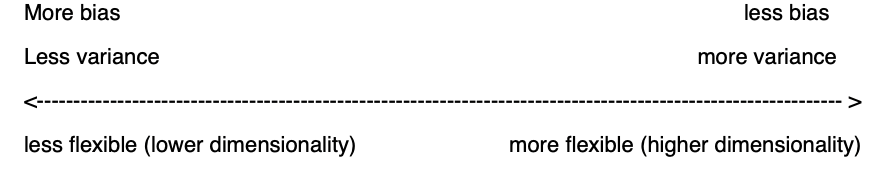
\includegraphics[scale=0.45]{img3}

3) (From Jupyter Notebook) \\
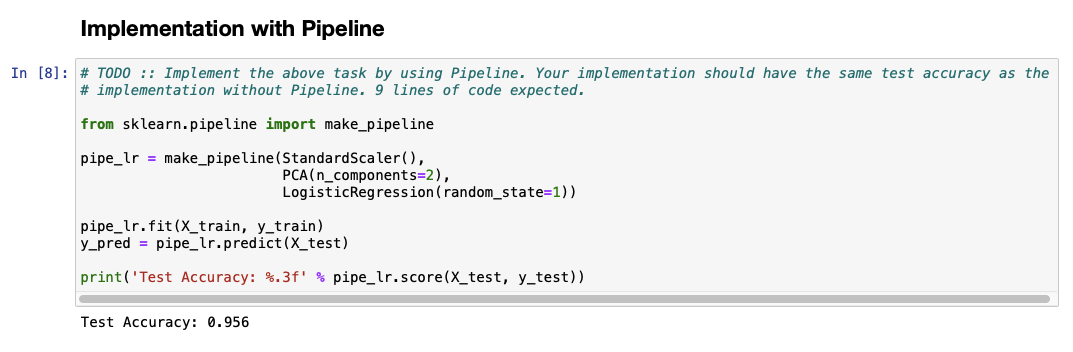
\includegraphics[scale=0.4]{code1} \\

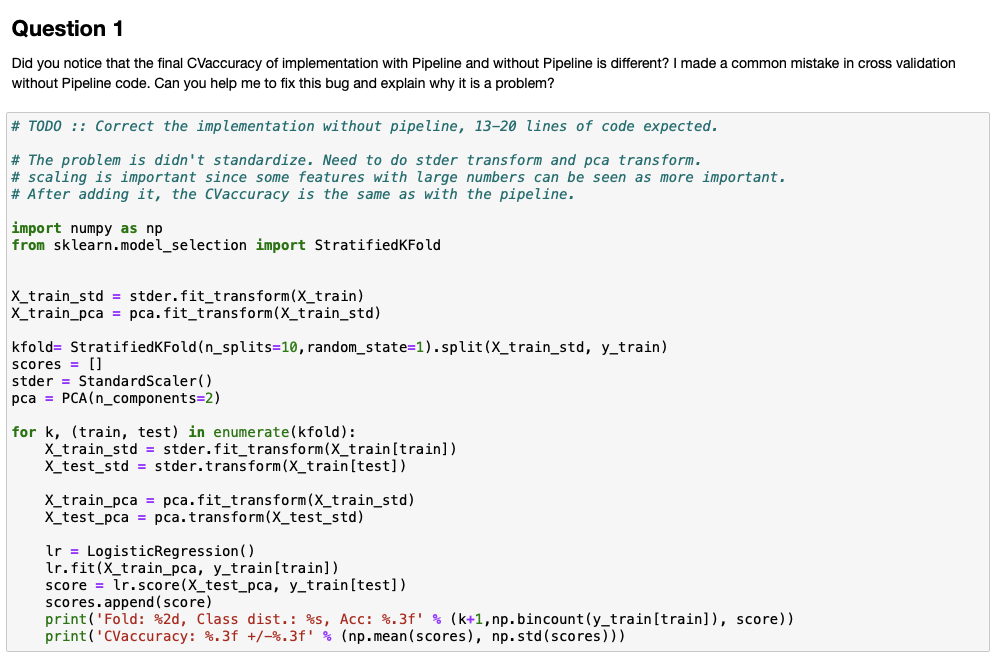
\includegraphics[scale=0.4]{code2} \\

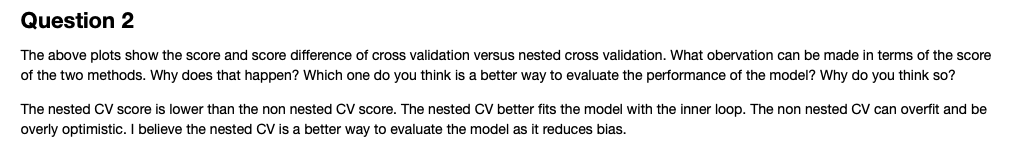
\includegraphics[scale=0.4]{code3} \\

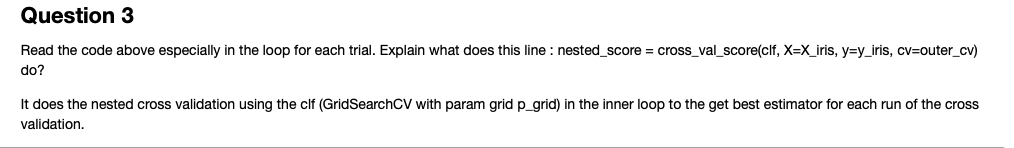
\includegraphics[scale=0.4]{code4} \\

\end{document}

